\documentclass{article}

% Important packages to use
\usepackage[utf8]{inputenc}
\usepackage{amssymb}
\usepackage{amsthm}
\usepackage{amsmath}
\usepackage[letter]{geometry}
\usepackage{graphicx}
\RequirePackage[12tabu, orthodox]{nag}
\usepackage{microtype} 	% impoves spacing
\usepackage{siunitx}	% simplify TeXing
\usepackage{cleveref}
\usepackage[colorlinks=false,pdforder={0 0 0}]{hyperref}


% Table of contents section
% -1 part     1 section     3 subsubsection  5 subparagraph
%  0 chapter  2 subsection  4 paragraph
\setcounter{tocdepth}{3}

% Automatic parenthesizing
% \usepackage{nath}
% \delimgrowth=1

% pseudocode
\usepackage{algorithmicx}
\usepackage{algpseudocode}

%%%%%%%%%%%%%%%%%%%%%%%%%%%%%%%%%%%%%%%%%%%%%%%%%%%%%%%%%%%%%
%%%%%%%%%%%%%%%%%%%%%%%%%%%%%%%%%%%%%%%%%%%%%%%%%%%%%%%%%%%%%
%%
%% TITLE 
%%
%%%%%%%%%%%%%%%%%%%%%%%%%%%%%%%%%%%%%%%%%%%%%%%%%%%%%%%%%%%%%
%%%%%%%%%%%%%%%%%%%%%%%%%%%%%%%%%%%%%%%%%%%%%%%%%%%%%%%%%%%%%
\title{Machine Learning}
\author{Teerapat (Mek) Jenrungrot}
\date{ }

\begin{document}
\maketitle

\tableofcontents

\section{Supervised Learning}
\subsection{Part I: Linear Regression}
Let $\theta_i$'s be the {\bf parameters} (also called {\bf weights}) paramaterizing the space of linear functions mapping from $\mathbb{X}$ to $\mathbb{Y}$. We make the notation, with $x_0 = 1$,

\begin{equation}
	\label{eq:hypothesis_function}
	h(x) = \sum_{i=0}^{n}\theta_i x_i = \theta^Tx
\end{equation}
as a hypothesis $h$ where on the right-hand side above we are vieweing $\theta$ and $x$ both as vectors, and here $n$ is the number of input variables (not counting $x_0$).

We now define the {\bf cost function}:
\begin{equation}
	\label{eq:cost_function}
	J(\theta) = \frac{1}{2}\sum_{i=1}^{m}(h_\theta(x^{(i)}) - y^{(i)})^2.
\end{equation}

\subsubsection{LMS algorithm}
\paragraph{gradient descent} We consider the {\bf gradient descent} algorithm, which starts with some initial $\theta$, and repeatedly performs update:
\begin{equation}
	\theta_j := \theta_j - \alpha\frac{\partial}{\partial \theta_j}J(\theta).
\end{equation}
Here, $\alpha$ is called the {\bf learning rate}. 
In order to implement this algorithm, we need to work out what is the partial derivative term on the right hand side. Let's first work it out for the case of if we have only one training example $(x,y)$, so that we can neglect the sum in the definition of $J$. We have:
\begin{align*}
	\frac{\partial}{\partial\theta_j}J(\theta) &= \frac{\partial}{\partial\theta_j}\frac{1}{2}(h_\theta(x)-y)^2 \\
	&= 2\cdot\frac{1}{2}(h_\theta(x)-y)\cdot\frac{\partial}{\partial\theta_j}(h_\theta(x)-y)\\
	&= (h_\theta(x)-y)\cdot\frac{\partial}{\partial\theta_j}\left(\sum_{i=0}^{n}\theta_ix_i-y\right) \\
	&= (h_\theta(x)-y)x_j
\end{align*}
Thus, for a single training example, this gives the update rule:
\begin{equation}
	\label{eq:update_rule}
	\theta_j := \theta_j + \alpha\left(y^{(i)}-h_\theta(x^{(i)})\right)x_j^{(i)}.
\end{equation}
\paragraph{batch gradient descent} This algorithm looks at every example in the entire training set on every step. 
\begin{algorithmic}
\Repeat 
	\State $\theta_j \gets \theta_j + \alpha \sum_{i=1}^{m}\left(y^{(i)} - h_\theta(x^{(i)})\right)x_j^{(i)}$
\Until{ it is convergence }
\end{algorithmic}
\paragraph{stochastic gradient descent} This algorithm updates the parameters according to the gradient of the error with respect to that single training example only. 
\begin{algorithmic}
\Loop
	\For{$i = 1$ to $m$}
		\State $\theta_j \gets \theta_j + \alpha \left(y^{(i)} - h_\theta(x^{(i)})\right)x_j^{(i)}$
	\EndFor
\EndLoop
\end{algorithmic}

\subsection{The normal equations}
In this section, we will discuss a second way of minimizing $J$ by using derivatives.
\subsubsection{Matrix derivatives}
\paragraph{$\nabla_A f(A)$} For a function $f: \mathbb{R}^{m \cross n} \rightarrow \mathbb{R}$, we define the derivative of $f$ with respect to $A$ to be:
\begin{equation}
	\label{eq:gradient_definition}
	\nabla_A f(A) = 
	\begin{bmatrix}
		\frac{\partial f}{\partial A_{11}} & \ldots & \frac{\partial f}{\partial A_{1n}} \\
		\vdots & \ddots & \vdots \\
		\frac{\partial f}{\partial A_{m1}} & \ldots & \frac{\partial f}{\partial A_{mn}}
	\end{bmatrix}
\end{equation}
\paragraph{trace operation} We define the {\bf trace} operator as:
\begin{equation}
	\label{eq:trace_definition}
	\text{tr} A = \sum_{i=1}^{n}A_{ii}
\end{equation}
We'll now prove that $\text{tr} (AB) = \text{tr} (BA)$ if $AB$ is square: 
\begin{align*}
	\text{tr} (AB) &= \sum_{i=1}^{n}(AB)_{ii} \\
	&= \sum_{i=1}^{n}\sum_{j=1}^{n}a_{ij}b_{ji} \\
	&= \sum_{j=1}^{n}\sum_{i=1}^{n}b_{ji}a_{ij} \\
	&= \sum_{j=1}^{n}(BA)_{jj} \\
	&= \text{tr} (BA)
\end{align*}
Followings are some more facts of matrix derivatives for if both $A$ and $B$ are square matrices:
\begin{align}
	\label{eq:gradient_equations}
	\nabla_A \text{tr} AB &= B^T \\
	\nabla_{A^T} f(A) &= \left(\nabla_A f(A)\right)^T \\
	\nabla_A \text{tr} ABA^TC &= CAB + C^TAB^T \\
	\nabla_A |A| &= |A| \left(A^{-1}\right)^T
\end{align}

\subsubsection{Least squares revisited}
\paragraph{design matrix} Given a training set, define the \textbf{design matrix} $X$ to be the $m$-by-$(n+1)$ matrix (including the intercept term) that contains the training examples' input values in its row:
\begin{equation}
	\label{eq:design_matrix}
	X = 
	\begin{bmatrix}
		- \left(x^{(1)})^T -\\
		- \left(x^{(2)})^T -\\
		\vdots \\
		- \left(x^{(m)})^T -\\
	\end{bmatrix}
\end{equation}
Let $\vec{y}$ be the $m$-dimensional vector containing all the target values from the training set:
\begin{equation}
	\label{eq:target_values}
	\vec{y} =
	\begin{bmatrix}
		y^{(1)} \\
		y^{(2)} \\
		\vdots \\
		y^{(m)} 
	\end{bmatrix}
\end{equation}
Now, since $h_\theta\left(x^{(i)}\right)^T\theta$, we can easily verify that
\begin{align*}
	X\theta - \vec{y} &= 
	\begin{bmatrix}
		\left(x^{(1)})^T\theta \\
		\left(x^{(2)})^T\theta \\
		\vdots \\
		\left(x^{(m)})^T\theta \\
	\end{bmatrix}
	-
	\begin{bmatrix}
		y^{(1)} \\
		y^{(2)} \\
		\vdots \\
		y^{(m)} 
	\end{bmatrix} \\
	&= 
	\begin{bmatrix}
		h_\theta\left(x^{(1)}\right) - y^{(1)} \\
		h_\theta\left(x^{(2)}\right) - y^{(2)} \\
		\vdots \\ 
		h_\theta\left(x^{(m)}\right) - y^{(m)} \\
	\end{bmatrix}.
\end{align*}
Thus, using the fact that for a vector $z$, we have that $z^Tz = \sum_{i}z_i^2$:
\begin{align*}
	\frac{1}{2}\left(X\theta - \vec{y}\right)^T\left(X\theta - \vec{y}\right) &= \frac{1}{2} \sum_{i=1}^{m}\left(h_\theta(x^{(i)}) - y^{(i)}\right)^2 \\
	&= J(\theta)
\end{align*}
Finally, to minimize $J$, we find its derivative with respect to $\theta$:
\begin{align*}
	\nabla_\theta J(\theta) &= \nabla_\theta \frac{1}{2}\left(X\theta - \vec{y}\right)^T\left(X\theta - \vec{y}\right) \\
	&= \frac{1}{2} \nabla_\theta \left( \theta^TX^TX\theta - \theta^TX^T\vec{y} - \vec{y}^TX\theta + \vec{y}^T\vec{y} \right) \\
	&= \frac{1}{2} \nabla_\theta \text{tr} \left( \theta^TX^TX\theta - \theta^TX^T\vec{y} - \vec{y}^TX\theta + \vec{y}^T\vec{y} \right) \\
	&= \frac{1}{2} \nabla_\theta \left( \text{tr} \theta^TX^TX\theta -2\text{tr}\vec{y}\right) \\
	&= \frac{1}{2} \left(X^TX\theta + X^TX\theta - 2X^T\vec{y}\right) \\
	&= X^TX\theta - X^T\vec{y}
\end{align*}
To minimize $J$, we set its derivative to zero, and obtain the {\bf normal equations}:
\begin{equation}
	\label{eq:normal_equation}
	X^TX\theta = X^T\vec{y}
\end{equation}
Thus, the value of $\theta$ that minimizes $J(\theta)$ is given in closed form by the equation
\begin{equation}
	\theta &= (X^TX)^{-1}X^T\vec{y}.
\end{equation}

\section{Statistical Learning}
\subsection{Measuring the Quantity fit}

\paragraph{Mean squared error}
The book defines the \textit{mean squared error} (MSE), given by
\[
	MSE = \frac{1}{n}\sum_{i=1}^{n}\left(y_i - \hat{f}(x_i)\right)^2
\]
where $\hat{f}(x_i)$ is the prediction that $\hat{f}$ gives for the $i$th observation. This value will be small if the predicted responses are very close to the true responses. Otherwise, the predicted value will be sunstantially high due to possibly bad predictors.

\paragraph{degree of freedom}
In short, \textbf{degree of freedom} describes the flexibility of a curve. The higher value of degree of freedom results in a highly fluctuating curve. 

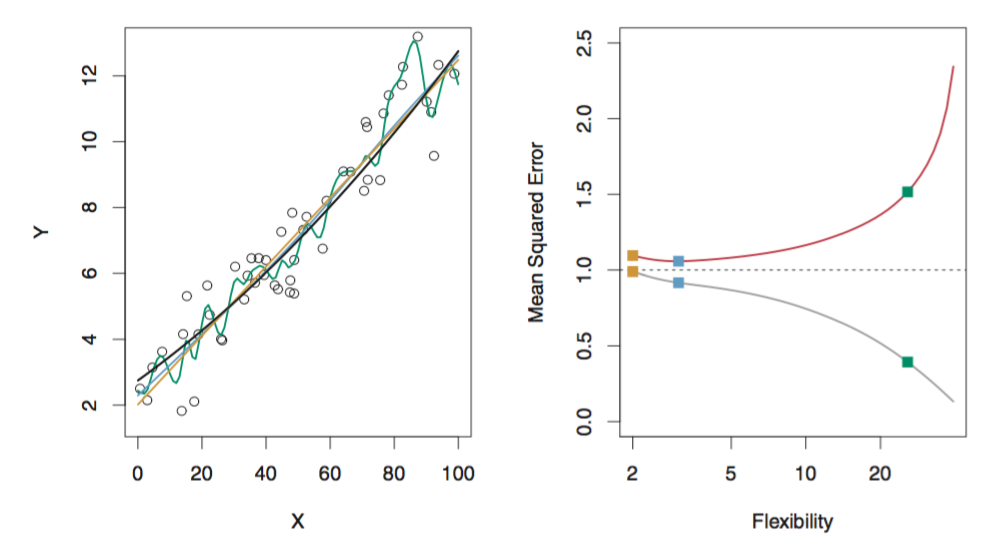
\includegraphics[scale=0.8]{images/flexibility_vs_mse.png} \\
This graph shows an example that the true $f$ is approximately linear. We observe that the training MSE decreases monotonically as the model flexibility increases, and that there is a U-shape in the test MSE. However, because the truth is so close to linear, the test MSE only decreases slightly before increasing again, so that \textbf{the orange least squares fit is substantially better than the highly flexible green curve}.  

\subsection{The Bias-Variance Trade-Off}
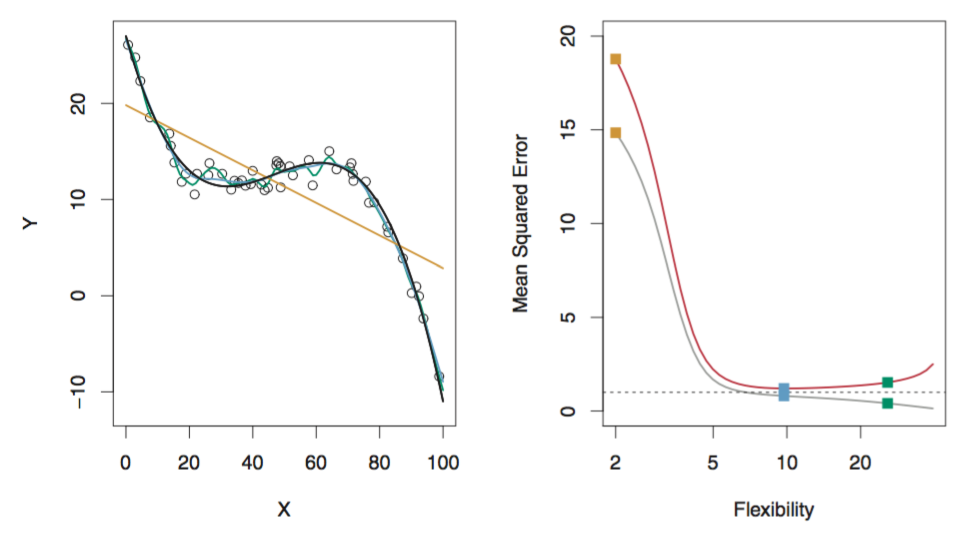
\includegraphics[scale=0.8]{images/linear_poorly_fits.png} \\
This graphs shows an example that the linear least square fit (as shown in the orange line) poorly fits the true $f$. 

\paragraph{Expected test MSE} It is possible to show that the \textbf{expected test MSE}, for a given value $x_0$, can always be decomposed into the sum of three fundamental quantities: the \textit{variance} of $\hat{f}(x_0)$, the squared \textit{bias} of $\hat{f}(x_0)$, and the variance of the error terms $\epsilon$. That is,
\[
	E\left(y_0 - \hat{f}(x_0)\right)^2 = \text{Var}(\hat{f}(x_0)) + \left[\text{Bias}(\hat{f}(x_0))\right]^2 + \text{Var}(\epsilon).
\]
We need to select a statistical learning method that simulataneously achieves low variance and low bias. 

\paragraph{Variance} Variance in this context refers to the amount by which $\hat{f}$ would change if we estimated it using a different training set. Since the training data are used to fir the statistical learning method, different training data sets will result in a different $\hat{f}$. But ideally the estimate for $f$ should not vary too much between training sets. However, if a method has high variance then small changes in the training data can result in large changes in $\hat{f}$. In general, more flexible statistical methods have higher variance. 

\paragraph{bias} On the other hand, \textit{bias} refers to the error that is introduced by approximating a real-life problem, which may be extremely complicated, by a much simpler model. For example, linear regression assumes that there is a linear relationship between $Y$ and $X_1, X_2, \ldots, X_p$. It is unlikely that any real-life problem truly has such a simple linear relationship, and so performing linear regression will undoubted result in some bias in the estimate of $f$. \textbf{As a general rule, as we use more flexible methods, the variance will increase and the bias will decrease}.

\subsection{The Classification Setting}
\paragraph{the training error rate} We define it as 
\[
	\frac{1}{n}\sum_{i=1}^{n}I(y_1 \ne \hat{y}_i).
\]
Here $\hat{y}_i$ is the predicted class label for the $i$th observation using $\hat{f}$. And $I(y_i \ne \hat{y}_i)$ is an indicator variable that equals 1 if $y_i \ne \hat{y}_i$ and 0 otherwise. A good classifier is one for which the test error is smallest.

\paragraph{The Bayes Classifier}
We classify data by assigning them to their most likely class, given thier predictor values. In other words, we should simple assign a test observation with predictor vector $x_0$ to the class $j$ for which
\[
	\text{Pr}(Y = j | X = x_0)
\]
is largest. To illustrate, in a two-class problem, the Bayes classifier corresponds to predicting class one if $\text{Pr}(Y = 1 | X = x_0) > 0.5$, and class two otherwise.

\paragraph{K-Nearest Neighbors}
In theory we would always like to predict qualitative responses using the Bayes classifier. But for real data, we do not know the conditional distribution of $Y$ given $X$, and so computing the Bayes classifier is impossible. K-nearest neighbors (KNN) classifier can solve such a problem. Given a positive integer $K$ and a test observation $x_0$, the KNN classifier first identifies the $K$ points in the training data that are closest to $x_0$, represented by $N_0$. It then estimates the conditional probability for class $j$ as the fraction of points in $N_0$ whose response values equal $j$:
\[
	Pr(Y = j | X = x_0) = \frac{1}{K}\sum_{i\in N_0}I(y_i = j).
\]
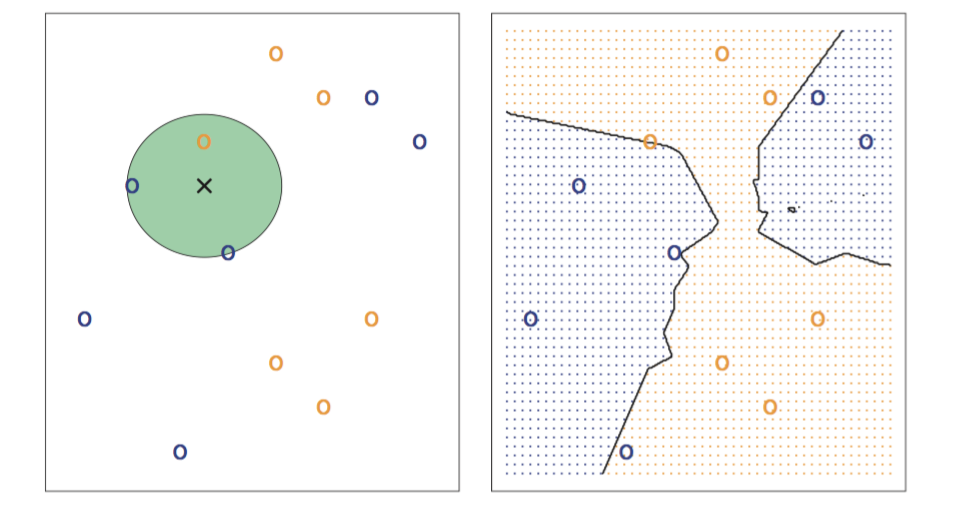
\includegraphics[scale=0.8]{images/knn1.png} \\ 

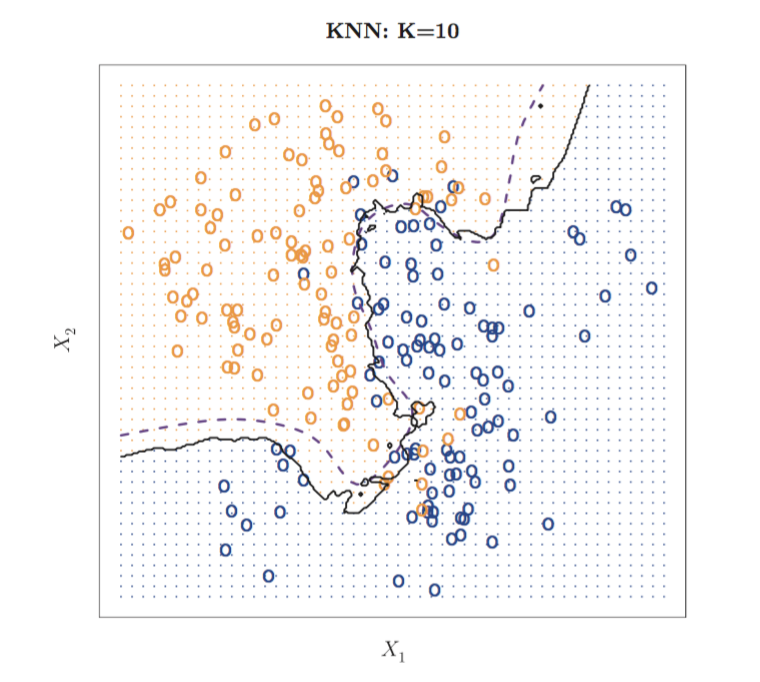
\includegraphics[scale=0.8]{images/knn2.png} \\ 
These images show the examples of KNN classifier.
\end{document}